\documentclass{article}
\usepackage[utf8]{inputenc}
\usepackage{graphicx}
\usepackage{biblatex}
\usepackage{tabularx}
\usepackage{graphicx}
\usepackage[table,xcdraw]{xcolor}
\usepackage{booktabs}
\usepackage{float}

\addbibresource{bibliography.bib}
\newcommand{\beginsupplement}{%
        \setcounter{table}{0}
        \renewcommand{\thetable}{S\arabic{table}}%
        \setcounter{figure}{0}
        \renewcommand{\thefigure}{S\arabic{figure}}%
     }
\title{Spatiotemporal dynamics of \textit{Streptococcus pneumoniae}}
\author{Sophie Belman}
\date{March 2021}

\begin{document}
\maketitle

\section{Abstract}
\textit{Streptococcus pneumoniae} is a globally distributed opportunistic bacteria commonly found in asymptomatic carriage but can cause invasive disease. It's diverse, comprising over 800 distinct sequence clusters with 100 serotypes and an open pangenome. Its global distribution and promiscuity lay the groundwork for constantly emerging phenotypes on genetic backbones with varying propensities for disease. Phylogeographic methods can be utilized to understand the global distribution and speed and breadth of spread, both overall and for distinct sequence clusters, which has implications for prevention and treatment campaigns. We have described the spatial structure of pneumococcal populations within the nine South African provinces and its rate of geographic spread across South Africa and to other countries. Optimizing time resolution methods will further improve the precision of our estimates. Incorporating transition matrices and variable allele frequencies between populations we are further working to describe the mechanistic drivers behind pneumococcal geographic transmission. 
147/200 words
\section{Background}
\subsection{Life History}
\textit{Streptococcus pneumoniae} (the pneumococcus) is an extracellular gram positive bacterium carried in the human upper respiratory tract (URT). Colonization with the pneumococcus has a range of outcomes from, asymptomatic carriage to, more rarely, life-threatening invasive pneumococcal disease (IPD)\cite{weiserStreptococcusPneumoniaeTransmission2018}. The pneumococcus was responsible for 55.5\%[95\% confidence intervals 36.07-76.05\%] of deaths from lower respiratory tract infection in 2019 and pneumococcal related deaths in 2015 were around 500,000\cite{wahlBurdenStreptococcusPneumoniae2018,murrayFiveInsightsGlobal2020}. There is known to be under detection in high-mortality developing countries due to limited access to care and testing making this a likely underestimate \cite{obrienBurdenDiseaseCaused2009,troegerEstimatesGlobalRegional2017}. 
\subsection{Vaccine} 
The globally implemented vaccine is a pneumococcal conjugate vaccine (PCV-13) targeting the 13 capsular serotypes (1, 3, 4, 5, 6A, 6B, 7F, 9V, 14, 18C, 19A, 19F, 23F) thought to be most ubiquitous in disease\cite{VaccineInformationStatement2019}. PCVs are designed to remove target serotypes from carriage in the nasopharynx to protect children, who represent the highest burden of disease, from pneumococcal infections \cite{bogaertStreptococcusPneumoniaeColonisation2004,wyllieMolecularSurveillanceStreptococcus2016}. PCV was broadly used in routine infant immunization programs in 146 countries by 2020 \cite{VaccineInformationStatement2019}. There was an estimated 51\% decline in pneumococcal related deaths globally from 2000 to 2015 and substantially reduced vaccine type associated pneumococcal disease among children both of which can be explained by implementation of PCV\cite{wahlBurdenStreptococcusPneumoniae2018, pilishviliSustainedReductionsInvasive2010,vongottbergEffectsVaccinationInvasive2014}. Over 100 capsular serotypes have been identified on genetic backbones of over 800 strains globally; called Global Pneumococcal Sequence Clusters (GPSCs)\cite{gladstoneInternationalGenomicDefinition2019b}. These will henceforth be interchangeably referred to as strains and GPSCs. The distribution of  GPSCs is not homogenous globally. In all sampled countries there are a low proportion of high frequency strains and high proportion of low frequency strains. High frequency GPSCs are more consistent between countries while low frequency GPSCs are more variable (Figure \ref{fig:gpscfreqdist}). This may be a result of some bias in sampling or may represent the presence of globally "Dominant" strains\cite{gladstoneInternationalGenomicDefinition2019b}.  
\begin{figure}
    \centering
    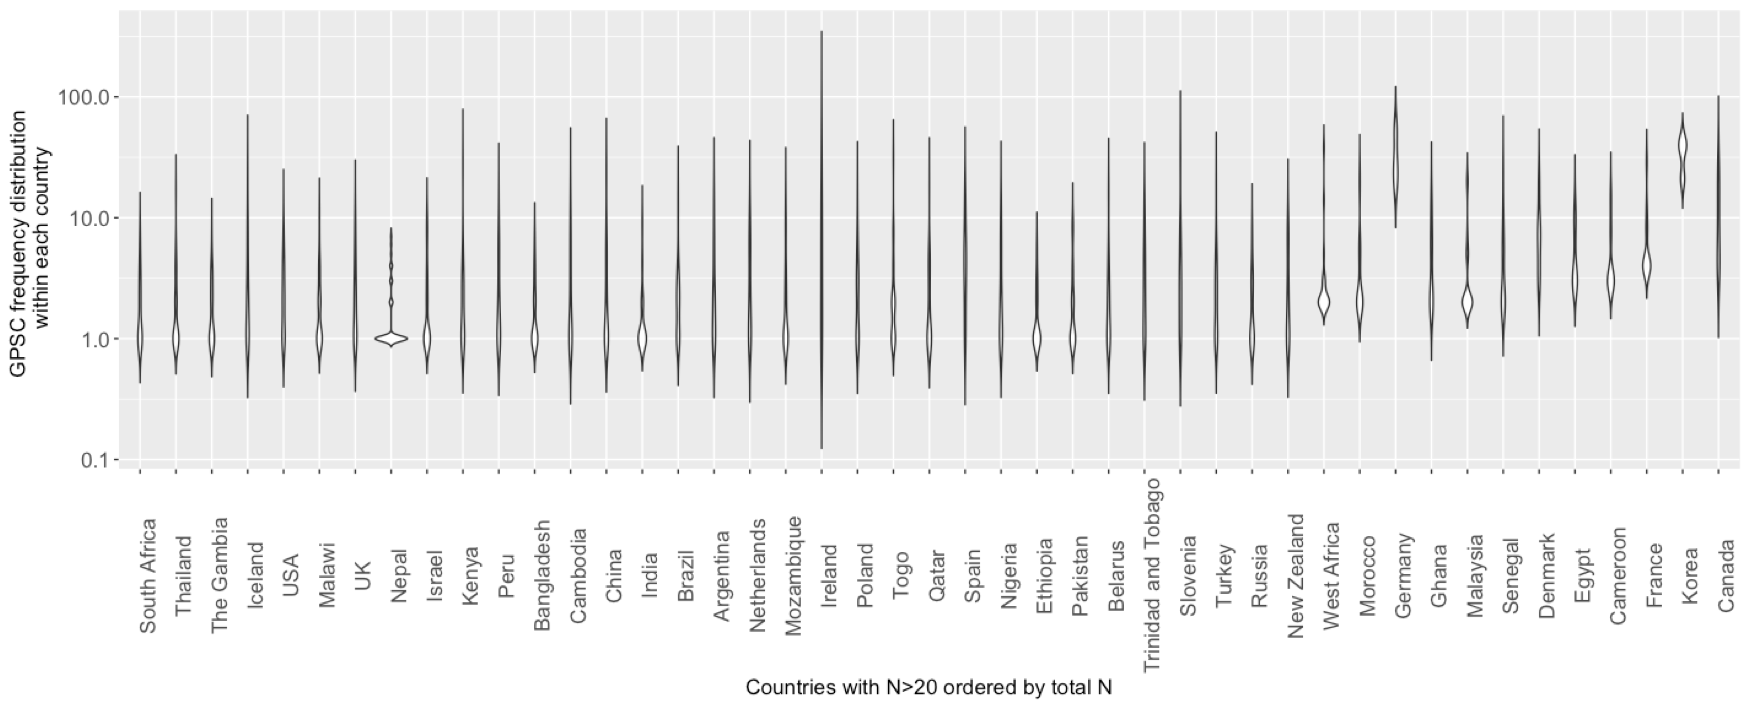
\includegraphics[width=\textwidth]{08MAR21_gpscfreqDistribution.png}
    \caption{Distribution of GPSC frequency by countries for which we have sampling of $N>20$}
    \label{fig:gpscfreqdist}
\end{figure} 
\\The pneumococcal genome is approximately 2Mbp and it is naturally competent for uptake of exogenous DNA. This natural competence results in homologous recombination both within and between species. It is not uncommon for GPSCs to undergo capsular switching between serotypes. Some GPSC’s have a propensity for high diversity of capsular types while others are restricted to a few \cite{loPneumococcalLineagesAssociated2019}. The reduction in vaccine types (VT) with the implementation of PCV clears the niche for expansion of non-vaccine types (NVT). This can perpetuate troublesome phenotypes such as antimicrobial resistance and association with IPD.
\subsection{Carriage \& Transmission} 
The pneumococcus colonizes mucosal surfaces in the upper respiratory tract, it promotes inflammation predominantly via pneumolysins which results in secretions and shedding. Close contact, co-occurrence with viral infections, and colder drier months all correlate with more likely transmission\cite{weiserStreptococcusPneumoniaeTransmission2018}. Rates of asymptomatic carriage in children under 5 range from 20-90\% with an inverse relationship with country income \cite{almeidaDynamicsPneumococcalCarriage2020,adegbolaCarriageStreptococcusPneumoniae2014}. The increased risk of adult carriage in households with children under 18 alongside children being the main reservoirs of pneumococcus, has resulted in children being considered the primary transmission vectors \cite{almeidaDynamicsPneumococcalCarriage2020,bogaertStreptococcusPneumoniaeColonisation2004}. A meta-analysis of lower-middle income countries indicated a wide range of carriage rates in adults from 8-85\% \cite{adegbolaCarriageStreptococcusPneumoniae2014}. Another study undertaken in the UK indicates a carriage prevalence of 20-40\% in adults\cite{almeidaDynamicsPneumococcalCarriage2020} . Carriage rates in adults is an under investigated topic likely due to the focus on the individuals with the greatest burden of disease --- children $<5$.  Carriage duration is estimated to be around 2 months but has been recorded for up to a year \cite{almeidaDynamicsPneumococcalCarriage2020,dubeLongitudinalCharacterizationNasopharyngeal2018}. The estimated generation time, time from infection to transmission, is estimated to be 1-2 months but is not well characterized and GPSCs carrying specific serotypes may be likely to be carried asymptomatically for a longer duration while others transmit more quickly\cite{leesGenomewideIdentificationLineage2017}.
\subsection{Phylogeographic analysis} 
Determining the speed and breadth of pneumococcal transmission requires estimates of divergence times between pairs. Phylogeographic methods have been used previously to estimate the historical dynamics of viruses, and some less diverse bacteria. For many studies phylogeographic methods are used to infer estimated time to emergence, patterns of introduction to specific regions, and mixing of geographically distinct populations\cite{wangGenomicEpidemiologyVibrio2020a,weillGenomicHistorySeventh2017,chihotaGeospatialDistributionMycobacterium2018,bartGlobalPopulationStructure2014,comasOutofAfricaMigrationNeolithic2013,allicockPhylogeographyPopulationDynamics2012,okoroIntracontinentalSpreadHuman2012,mutrejaEvidenceSeveralWaves2011,lemeyBayesianPhylogeographyFinds2009a}. Existing methods require building accurate phylogenies in which branch lengths, normally comprising mutation accumulation, are converted to divergence times. This is complicated by the diversity and high recombination rates of the pneumococcus, as substitutions (estimated to be approximately $1.57X10^-6$ substitutions per site per year; 3.14 SNPs per genome per year) account for a smaller proportion of the mutations in its genome than sites which have undergone recombination \cite{croucherRapidPneumococcalEvolution2011}. To resolve this in the pneumococcus we mask recombinatory sites, which although successful, may result in clock rate estimates based on a smaller proportion of genome than in species without recombination. Recombination masking in highly recombinatory bacteria can produce spurious signals of population growth and skew clock rate estimates, however, BEAST and BactDating, two examples of time resolution software using Bayesian inference methods are robust for root estimates as well as relative divergence times\cite{cornickRegionspecificDiversificationHighly2015,gladstoneInternationalGenomicDefinition2019b,croucherRapidPhylogeneticAnalysis2015,didelotBayesianInferenceAncestral2018,drummondBayesianEvolutionaryAnalysis2015,lapierreImpactSelectionGene2016}. As in Cornick et. al 2015 estimates of divergence times successfully demonstrated region specific diversification and cross region transmission of a specific pneumococcal serotype\cite{cornickRegionspecificDiversificationHighly2015}.
Didelot et. al 2018 performed benchmarking for several time resolution methods using the pneumococcus demonstrating concordance and giving further credence to their use in pneumococcal investigations\cite{didelotBayesianInferenceAncestral2018}. However, estimates which require more precise time estimates such as time from emergence to mixing in a geographic region, variability in the geographic rate of spread overall and between strains, have not yet been explored.  
\subsection{Global Pneumococcal Sequencing Project (GPS)}
The Global Pneumococcal Sequencing Project (GPS) is a global genomic survey of \textit{Streptococcus pneumoniae}. GPS has partners in over 50 countries and has sequenced ~30K  genomes to date (March 2021). These comprise both carriage and disease isolates with an over representation of children under 5 but some inclusion of adult samples.
\subsection{Ancient Genome }
Ancient genomes have been used to contextualize the phylogeographic history of several bacteria including \textit{Mycobacterium tuberculosis} and \textit{Salmonella typhi}\cite{bosPreColumbianMycobacterialGenomes2014,vageneSalmonellaEntericaGenomes2018}. The ancient DNA field is continuing to expand as more ancient genomes are successfully sequenced \cite{neukamm2000yearoldPathogenGenomes2020}. The identification of \textit{S. pneumoniae} in a 5700 year old metagenome on the island of Syltholm in Denmark provided an opportunity to elucidate thousands of years of evolutionary context for extant strains\cite{jensen5700YearoldHuman2019}. 
987/1200
\section{Aims}
\subsubsection{The question of migration} 
The diversity of the pneumococcus, duration of carriage, and unclear drivers of transmission as well as its highly recombinatory genetic backbones and serotypes, entreats questions of geographic spatial structure and migration, especially with regards to expanding and emerging phenotypes. Some of the questions I work towards answering in this section include:
\\
\\1) What is the resolution to which there is there geographic spatial structure --- continents, countries, provinces? 
\\2) Are there differences in transmission rate between GPSCs which are restricted to geographic regions and those which maintain prevalence globally?  
\\3) Can an ancient genome be used to elucidate when GPSCs diverged and how long have they been circulating? 
\\
\\As has been demonstrated with the rapid spread of SARS-CoV2 in 2020-2021 our global populations are not isolated. We are a highly interconnected world not just sharing goods and ideas but sharing pathogens as well. Answering these questions with regard to the pneumococcus will help to elucidate the potential impact of vaccine and antimicrobial derived selection pressure on the global spread of expanding and emerging phenotypes. 
175/200
\section{Methods}
\subsection{South African Phylogeography}
\subsubsection{South African Pneumococcal Collection and Sequencing}
We included genomes from GPS  collected in South Africa predominantly in this study. We also included global genomes which were the focus GPSCs for context. We utilized metadata including collection year and month, residence province of the patient, age of the patient, sampling site, and clinical manifestation. The South African samples were isolates from a range of sampling sites and clinical manifestations. These included nasopharyngeal swabs, blood, pleural fluid, cerebrospinal fluid, peritoneal fluid, pus, and other joint fluid. We inferred carriage or disease from a combination of sampling site and clinical manifestation information.
These samples were selectively cultured on BD™ Trypticase™ Soy Agar II with 5\% sheep blood (Beckton Dickinson, Heidelberg, Germany) and incubated overnight at 37 °C in 5\% CO2. Genomic DNA was then extracted manually using a modified QIAamp® DNA Mini Kit (QIAGEN, Inc., Valencia, CA) protocol. As part of the Global Pneumococcal Sequencing (GPS) Project, pneumococcal isolates were whole-genome sequenced on the Illumina HiSeq platform to produce paired-end reads with an average of 100-125 bases in length and data were deposited in the European Nucleotide Database. WGS data was processed as previously described\cite{gladstoneInternationalGenomicDefinition2019b}.
\subsubsection{Mitigating Sampling Bias}
To compensate for sampling bias imposed by the uneven sampling across different South African provinces we scaled the data set to N=50 for each province and GPSC. When the number of a unique GPSC in each province was less than 50 we included all without replacement. When the number of a unique GPSC in a given province was greater than 50 we sampled without replacement to 50. Uncertainty was determined via bootstrapping. We performed a sensitivity analysis to assess the impact of different sampling strategies including weighted sampling and varying the N to which we scaled the data set.  
\subsubsection{Tree Building}
We selected only GPSCs for which we had genomes from each of South Africa's nine provinces to build phylogenies, henceforth referred to as "focus GPSCs". We created reference genomes for each GPSC using ABACAS to order the contigs from a representative of each GPSC to \textit{Streptococcus pneumoniae }(strain ATCC 700669/Spain 23F-1) [EMBL accession: FM211187]\cite{assefaABACASAlgorithmbasedAutomatic2009}. Any contigs which did not align were concatenated to the end.  We multiply mapped all representatives against these references using a custom mapping, variant calling, and local realignment around indels pipeline using bwa-MEM \cite{liFastAccurateShort2009}, and samtools mpileup\cite{liFastAccurateShort2009}. We built trees masking recombinatory regions using gubbins\cite{croucherRapidPhylogeneticAnalysis2015} and a GTR model. The collection dates for the tips of the trees were compiled. We converted branch length to time using BactDating with a mixed gamma, relaxed clock model \cite{didelotBayesianInferenceAncestral2018}. To evaluate accuracy BactDating time resolution we used BEAST both strict and relaxed clocks and a Bayesian skyline prior to compare for concordance.
\subsubsection{Statistical methods}
We built a framework using the odds ratio to investigate the impact of genetic distance and geographic distance on likelihood of similarity where for all pairs \textit{r=same province}, \textit{t=same collection time}, \textit{s=same GPSC} (Equation \ref{equat1}). We performed to strain level designation to determine whether GPSCs circulated homogenously across South Africa, or if there were distinct GPSCs in different provinces. 
\begin{equation}
\frac{\frac{(r*t)*s}{r*t}}{\frac{(1-r)*t*s}{(1-r)*t}}
\label{equat1}
\end{equation}
We then utilized the aforementioned time resolved phylogenetic trees to increase the genomic distance resolution. We converted the time resolved trees to pairwise divergence time matrices. Geographic distances were calculated based on the centroid latitude and longitude of each province. We performed pairwise comparisons across a range of genomic distances determining the mean geographic distance between pairs separated by a specified divergence time. We built these curves overall and for each focus GPSC. We fit an isotropic transmission model to the curve to determine the rate of geographic spread across South Africa as described in Equation 5 of Salje et. al. 2016 \cite{saljeEstimatingInfectiousDisease2016}. \\We utilized the same framework to increase the geographic resolution and compare a range of geographic distances where $des_r=$\textit{designated pairwise geographic distance} and  $ref_r=$ \textit{reference pairwise geographic distance}(Equation \ref{equat2}). We did this for both the strain level designation and the higher genomic distance resolution conferred from the phylogenies.
\begin{equation}
\frac{\frac{(des_r*t)*s}{des_r*t}}{\frac{(ref_r)*t*s}{(ref_r)*t}} 
\label{equat2}
\end{equation}
To increase the genomic distance resolution in equation \ref{equat2}, where \textit{s} previously indicated whether a pair were the same GPSC instead we evaluated likelihood of a specified divergence time across geographic distances where \textit{s=designated tMRCA range} (time to most recent common ancestor), and all else in equation \ref{equat2} is the same. To determine how long homogenization across South Africa takes we investigated the divergence time at which there was no increased odds of similarity within a province compared against distance provinces (OR=1). \\
Additional to the South Africa analysis I built a pipeline and characterized a previously un-described ancient streptococcal genome from Denmark. 
All statistical analysis was performed in R v3.6.2
734/500
\section{Results}
\subsection{Spatiotemporal dynamics of the pneumococcus in South Africa}
We utilized isolates from South Africa for this analysis (N=6920). These were from nine provinces Gauteng (N=3171), Mpumalanga (N=1308), Western Cape (N=880), KwaZulu-Natal (N=649), Free State (N=347), Eastern Cape (N=300), North West (N=116), Northern Cape (N=80), and Limpopo (N=69). In total these comprised 196 GPSCs with 69 different serotypes (Figure \ref{fig:map}). 
\begin{figure}[H]
\centering
    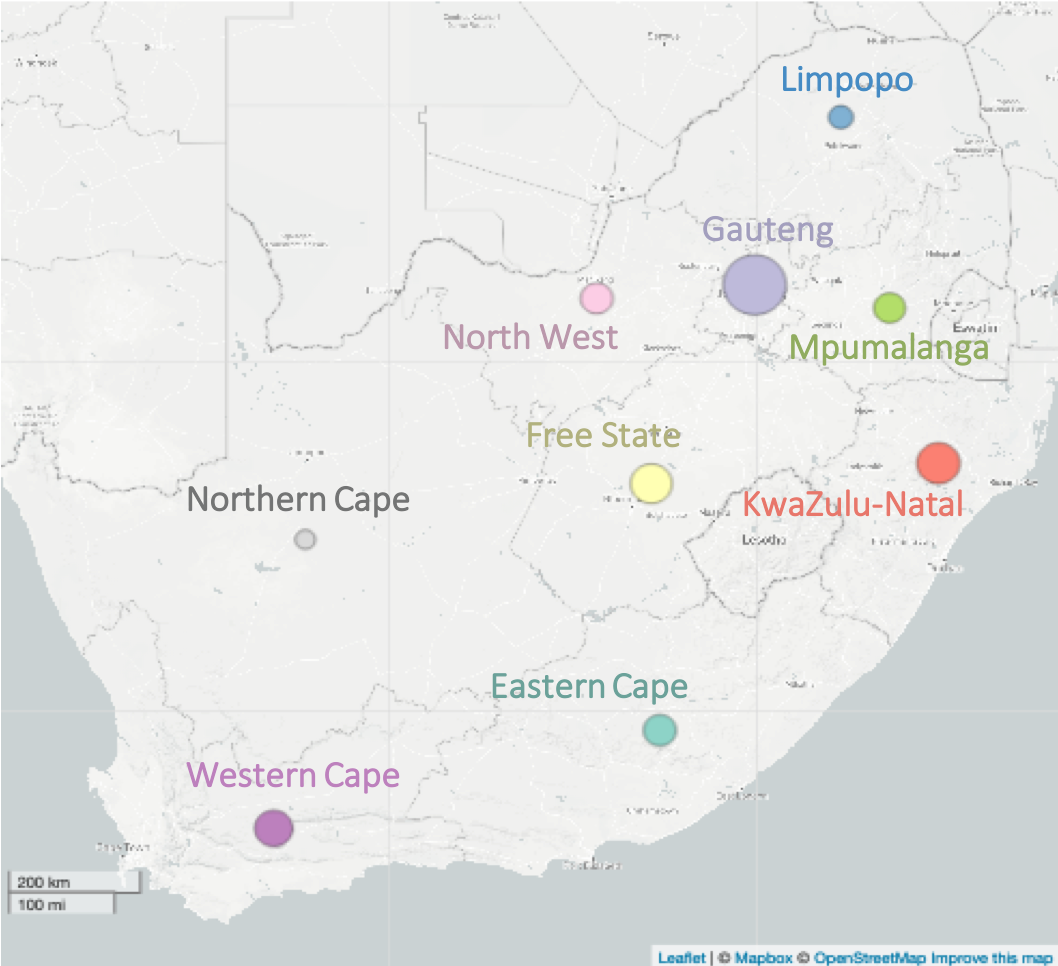
\includegraphics[width=\textwidth]{scaledmap.png}
    \caption{Map of nine provinces of South Africa scaled to sampling for each province for the nine GPSCs with representatives in each province}
    \label{fig:map}
\end{figure}
\\To determine whether there was spatial structure with distinct GPSCs circulating in specific provinces we constructed pairwise matrices for each province comprising every genome from that province compared with every other genome in the data set. We then determined the proportion of genomes which were the same GPSC as another in the same province compared to the proportion which were the same GPSC as a genome from a different province (Equation \ref{equat1})(Figure \ref{fig:withinbetween}B). Dividing the proportion which are the same within province by the proportion between provinces which are the same garners the odds ratio (Figure \ref{fig:withinbetween}A). These ranged from no increased risk of distinct GPSC pairs circulating in Limpopo (OR=1.09 [95\%CI 0.64-1.57]) to 1.46 (95\%CI 1.37-1.53) times as likely in Western Cape (Figure \ref{fig:withinbetween}A). There was no clear correlation between provinces with higher likelihood of distinct GPSCs within province and any other demographic factors including population size, area, GDP, or number of borders (Figure \ref{fig:withinbetween}C). We performed a sensitivity analysis for sub-sampling (Figure \ref{fig:sensanalysis}).
\\This method demonstrated resolution to the strain level using a simple categorization of whether or not a pair are the same strain or different strains. Resolving the time to the most recent common ancestor (tMRCA) between pairs allows higher resolution analysis. Rather than asking whether a pair is the same strain, asking has a pair diverged within a year, within 5 years, within 15 years --- with an infinite number of possible divergence times to be explored across a continuous scale. 
\begin{figure}[H]
\centering
    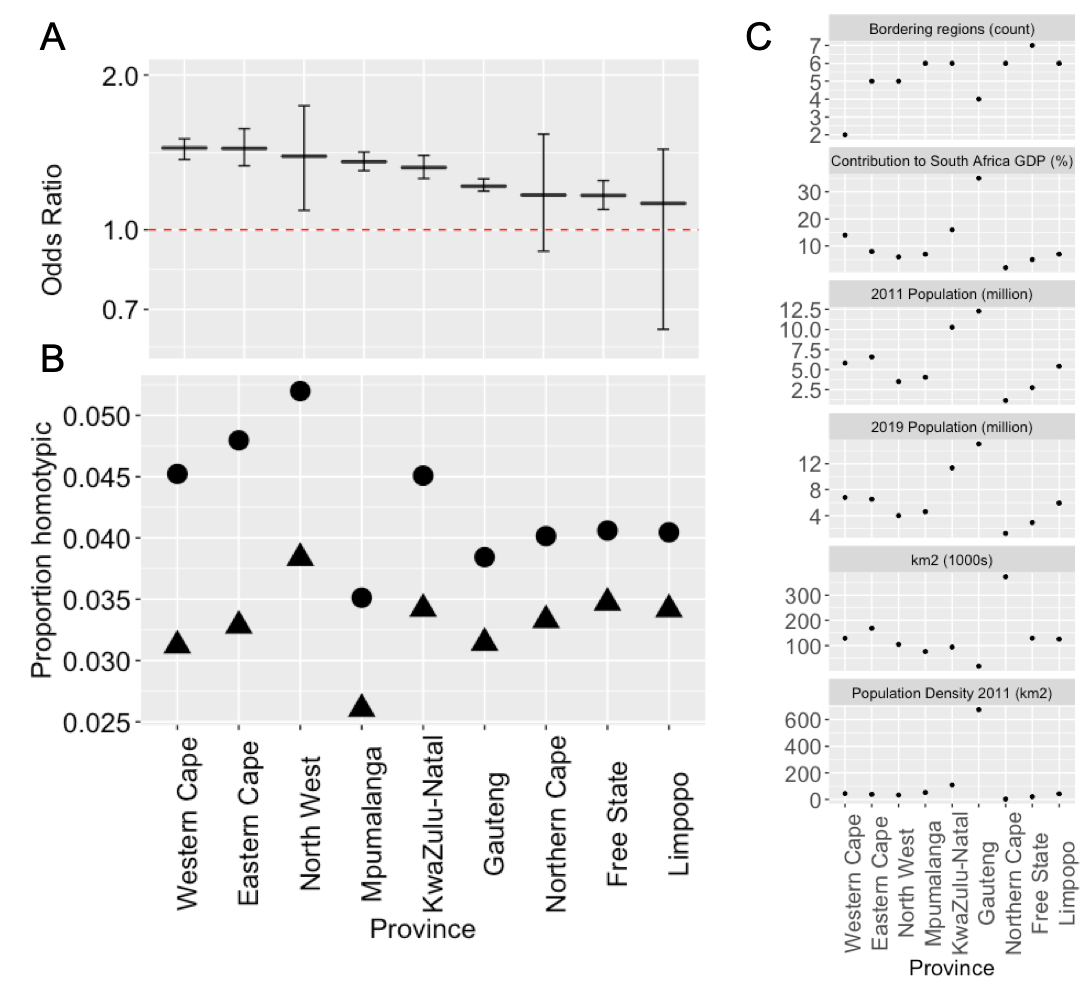
\includegraphics[width=\textwidth]{withinvsbetween.png}
    \caption{Specificity of GPSCs within each province A) Odds that the GPSCs circulating within each province (shared x-axis with B) are more similar to those with the same province or those from other provinces for each province. B) Proportion which are homotypic (same GPSC) within each province (circles) to those which are homotypic from different provinces (triangles). C) Characteristics of each province plotted in the same order as for A and B comprising the number of bordering regions, the provinces contribution to South Africas GDP, the population in 2011, the population in 2019, the area in km2, and the population density in 2011.}
      \label{fig:withinbetween}
\end{figure}
The focus GPSCs  (N=5195 ; South Africa N=2579) included: GPSC2 (N=1113; South Africa N= 507), GPSC17 (N=491; SA N= 463), GPSC14 (N=503; SA N=413 ), GPSC13 (N=508; SA N=308 ), GPSC5 (N=721; SA N=304 ), GPSC10 (N=462; SA N=236 ), GPSC1 (N=1228; SA N=199 ), GPSC79 (N=90; SA N=86 ),  and GPSC68 (N=79; SA N=64 ). We determined the mean pairwise geographic distance for pairs within specific evolutionary distances (cumulative) (Figure \ref{fig:transrate}A) and the rate of geographic spread didn't exceed the 95\% confidence intervals (CIs) of the overall curves for any GPSCs indicating a similar rate of geographic spread by this method(Figure \ref{fig:transrate}B). To minimize the impact of any spatiotemporal sampling biases we only considered pairs which were collected within a year of each other. We fit a simple model to the overall curve (Figure \ref{fig:transrate}A) which indicated a geographic rate of spread of 54.28 (95\% CIs  45.69-67.11) km/year. 

\begin{figure}[H]
\centering
    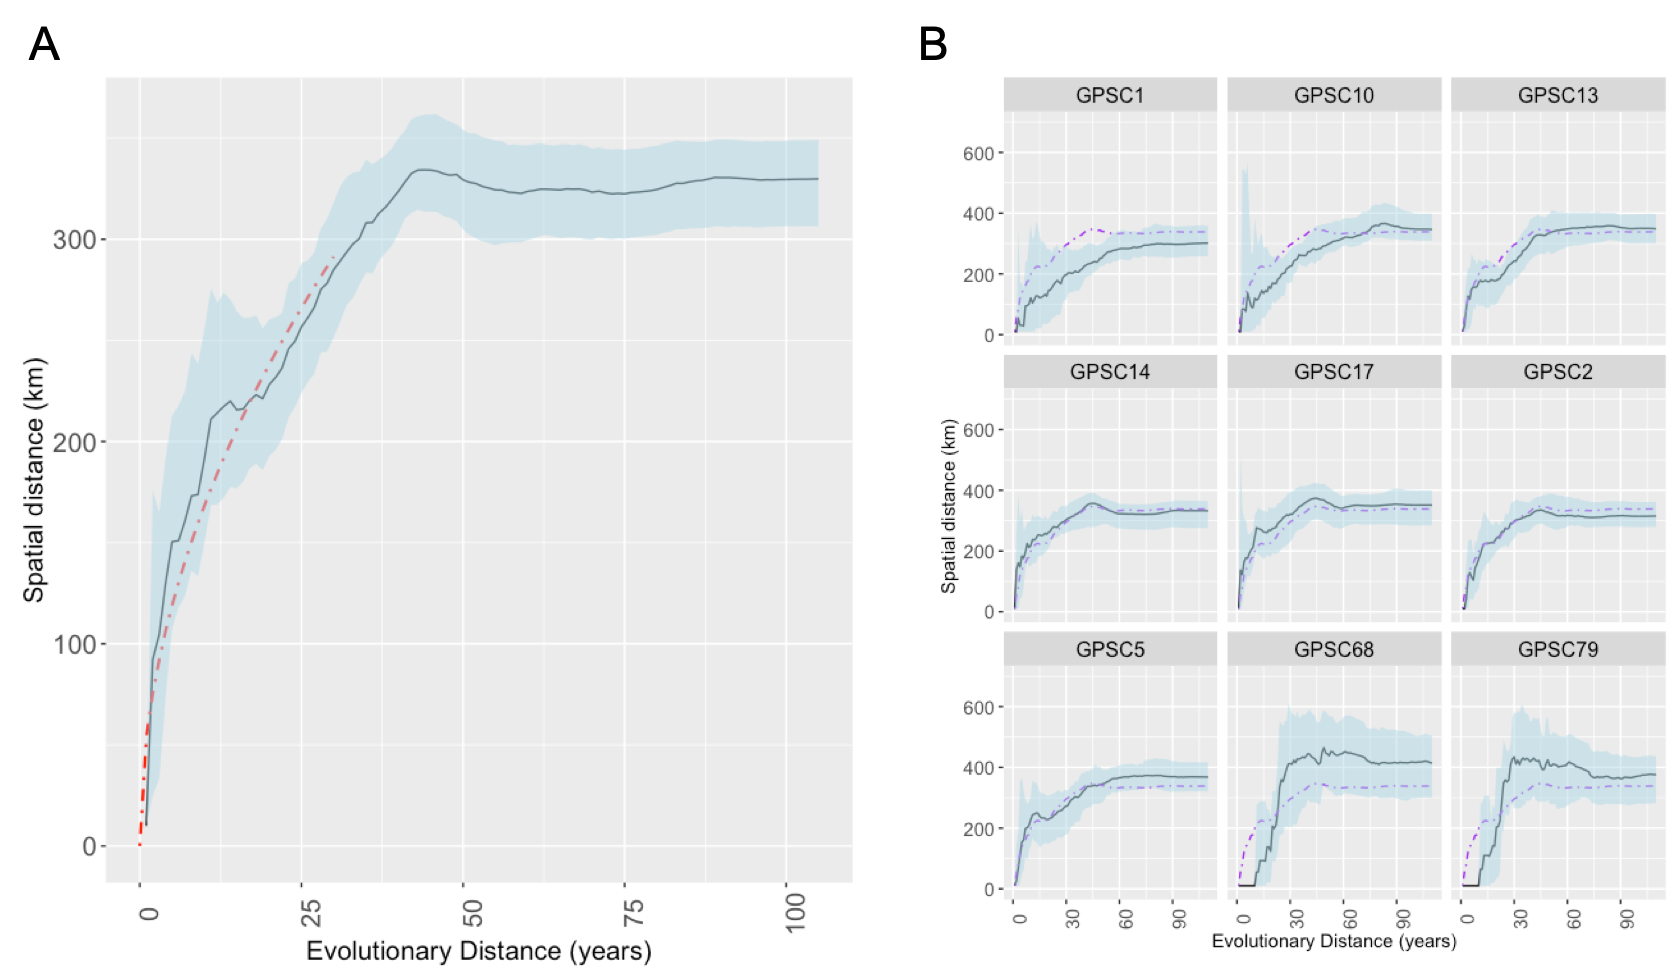
\includegraphics[width=\textwidth]{transrate_AB.png}
    \caption{The mean geographic distance (km) for pairs with specified cumulative evolutionary distance (years) for A) all GPSCs with a representative in each of the nine provinces combined (N=5195) and for B) each GPSC individually}
      \label{fig:transrate}
\end{figure}
\\The correlation between increasing geographic distance evolutionary distance is expected and we wanted to interrogate this more specifically on different spatial scales. Is there a steady rate of mixing or do borders such as those between provinces inhibit geographic spread. To determine the likelihood of similarity between pairs over an increasing scale of geographic distances we used discrete distances including: pairs from within the same province, from different provinces but $<$400km apart, between 400 and 700 km apart, from 700 to 1000km apart, to over 1000km apart, pairs in which one was from South Africa and one was from another African country, and one from South Africa with one from a country outside of Africa. We used distant pairs from South Africa ($>$1000km apart) as a reference. We performed this both at low resolution where \textit{s=same GPSC} (Figure \ref{fig:strainvstmrca}A),
\begin{figure}[H]
\centering
    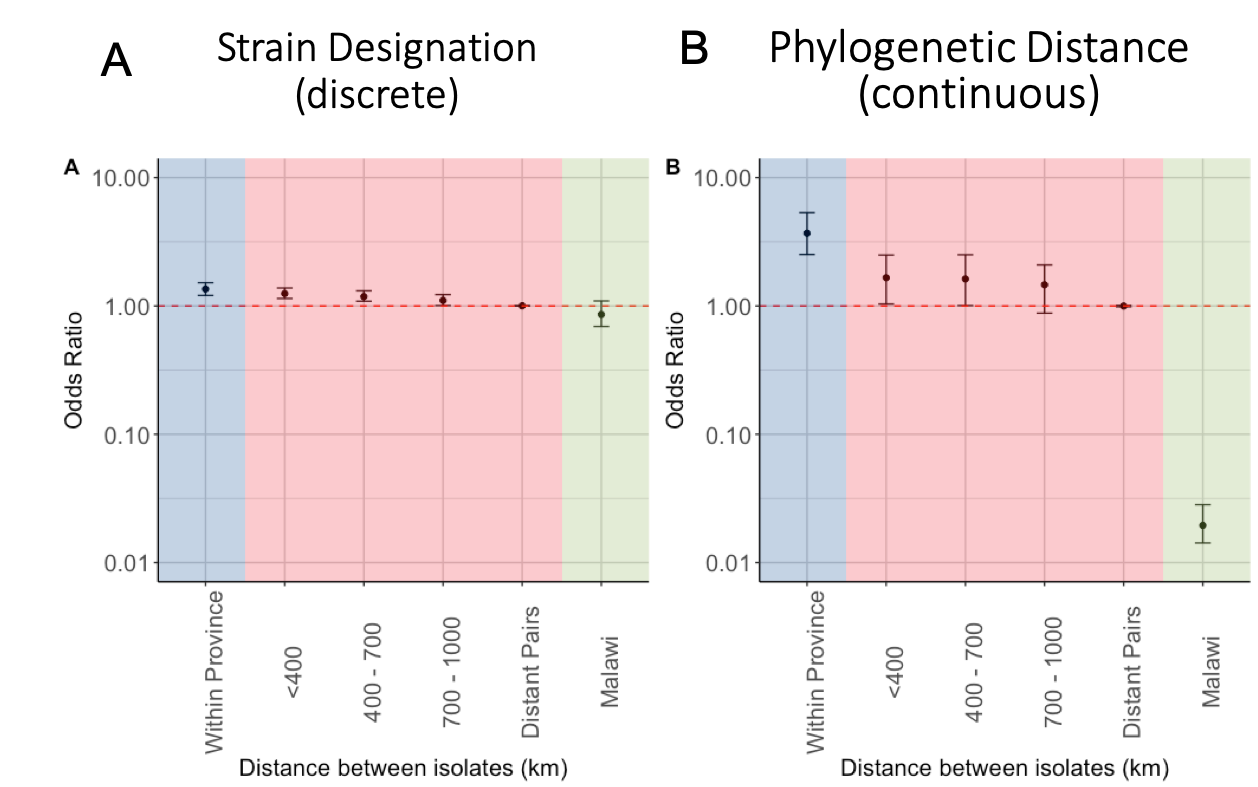
\includegraphics[width=\textwidth]{strainvstmrca.png}
    \caption{Likelihood of either A) being the same GPSC/strain or B) having tMRCA within 3 years within a province (blue), between different provinces over increasing distance (red), and pairs from South Africa and Malawi (green), using geographically distant pairs ($>$1000km) as a reference.}
      \label{fig:strainvstmrca}
\end{figure}
and high resolution where \textit{s=designated tMRCA}(Figure \ref{fig:strainvstmrca}B).  There is an increased signal conferred by evaluating divergence time between pairs rather than whether they are the same strain. When using a reference of pairs collected from different provinces it is 1.30 (95\% CI 1.18- 1.43) times as likely that a pair collected from within the same province will be the same GPSC (Figure \ref{fig:strainvstmrca}A); whereas it is 4.69 (95\%CI 3.37-7.36) times as likely that pairs from within the same province have a most recent common ancestor (tMRCA) within the past three years (Figure \ref{fig:strainvstmrca}B). As the time to divergence increases the increased likelihood of similarity conferred by proximity decreases (Figure\ref{fig:timedistance}A). There is a larger decreased likelihood when comparing pairs from within a province to pairs from different provinces than the decreased likelihood of increasing distances between those different provinces. \\It takes 50 years for a strains to become homogenously mixed across South Africa (Figure \ref{fig:timedistance}B). Furthermore, there is  a steadily increasing odds that a pair of genomes from South Africa and another African country, as well as pairs from South Africa and a country outside of Africa, will have similar divergence times to distant South African pairs. This reaches nearly equal odds when divergence time reaches 100 years (Figure\ref{fig:timedistance}B). 
\begin{figure}[H]
\centering
    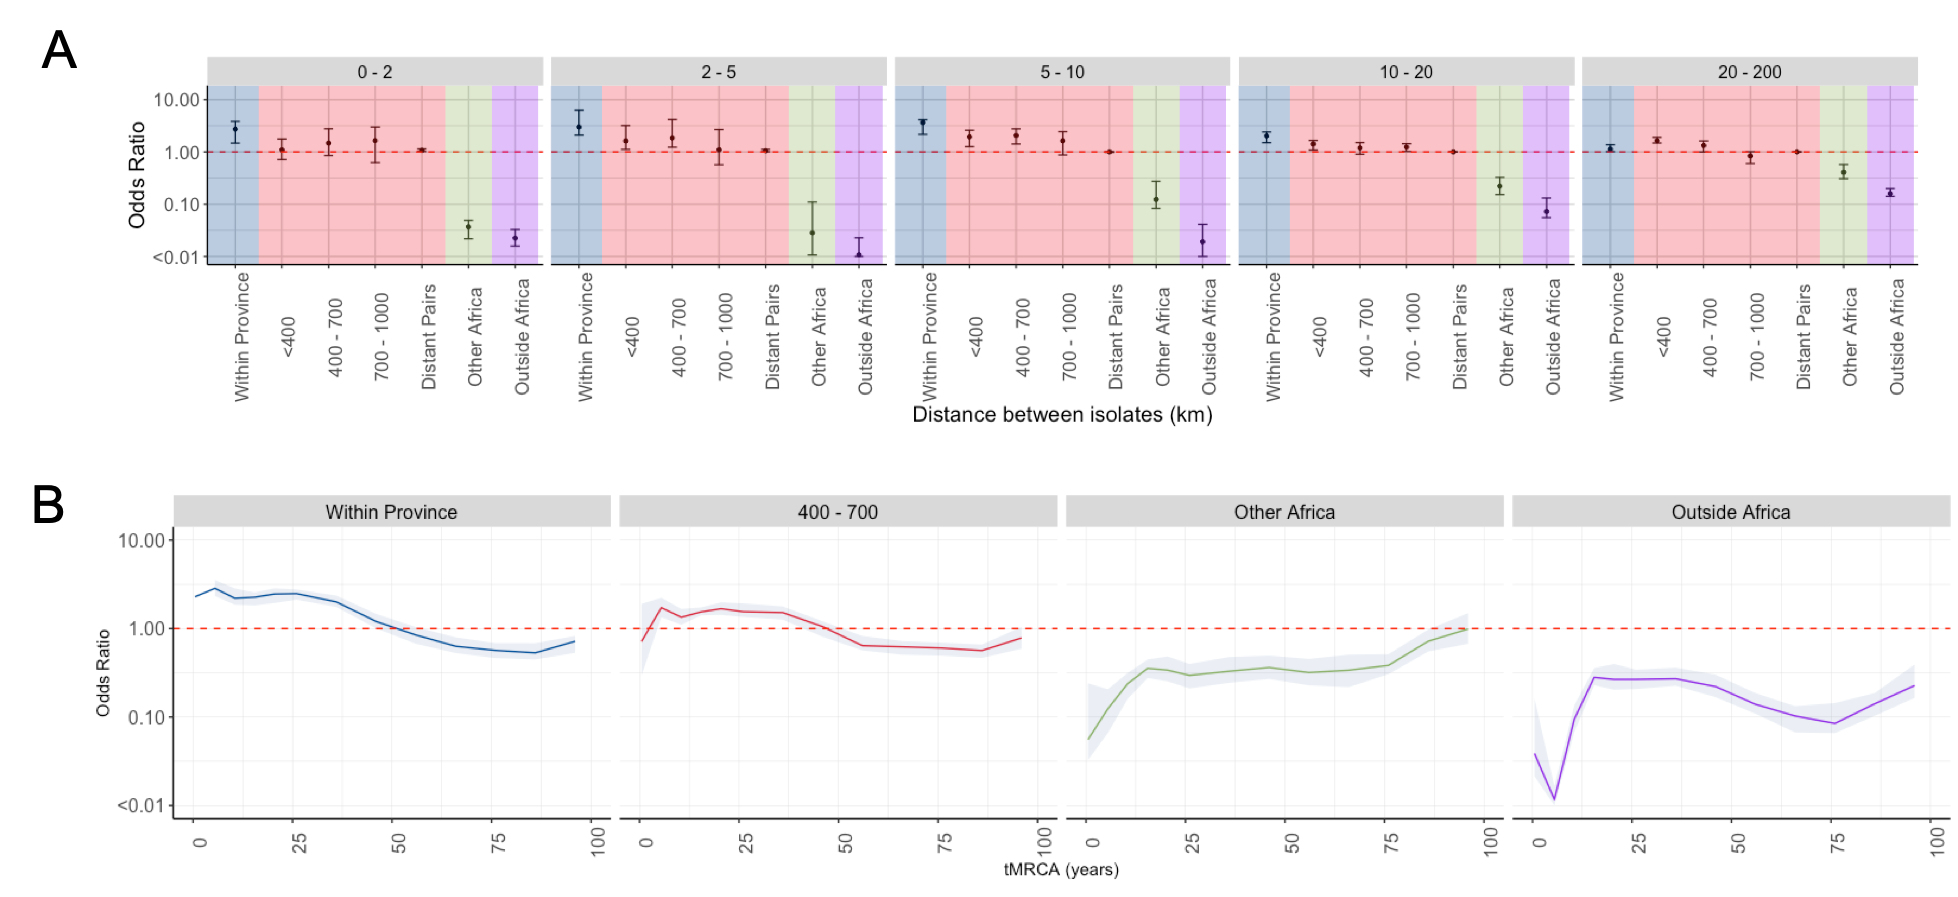
\includegraphics[width=\textwidth]{timeanddistance.png}
    \caption{Likelihood of having tMRCA a A) 0-2,2-5,5-10,10-20,20-200 within South African provinces (blue), across larger distances within South Africa (red), from South Africa to other countries in Africa (green), and from South Africa to countries outside of Africa (purple) or B) across a range of tMRCAs in 50 year windows plotted at the median from 0-100 with the same color specifications as A. Both A and B use a reference of pairs which are from distant provinces in South Africa. Subsampled to 50 with replacement using 9 time resolved trees of GPSCs (N=5195).}
      \label{fig:timedistance}
\end{figure}
\begin{figure}[H]
\centering
    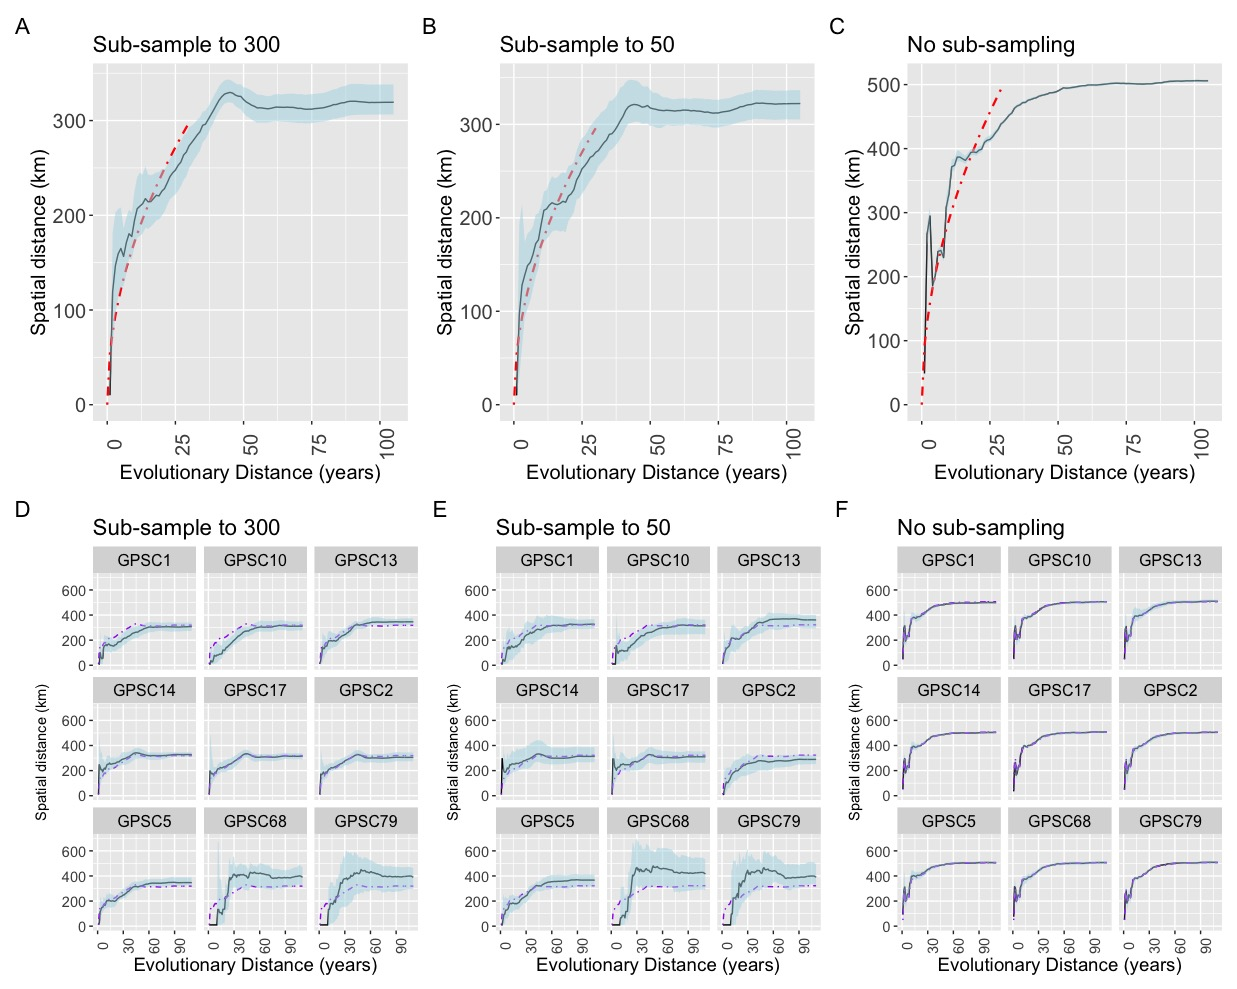
\includegraphics[width=\textwidth]{sensitivity_sampling.jpeg}
    \caption{Sensitivity of sampling methods A \& D) Sub-sampling to 300; B \% E) Sub-sampling to 50; and C \& F) involve no sub-sampling and have obvious peaks of over represented distanced. This demonstrates the value of mitigating sampling bias by scaling the data set.}
      \label{fig:sensanalysis}
\end{figure}
\subsection{Characteristics of an ancient streptococcal genome }
We worked to extract all pneumococcal reads from the ancient metagenome to contextualize it with extant strains and determine its potential pathogenicity. In brief, metagenome data was generated from an ancient birch pitch sample discovered on the Syltholm island of Denmark by Jensen et. al. at the University of Copenhagen\cite{jensen5700YearoldHuman2019}. Dr. Jonas Niemann kindly shared the metagenome data with us after the aligned human reads were removed. A content report generated using kraken2 v2.0.8 and bracken v2.5.2 \cite{KrakenUltrafastMetagenomic,luBrackenEstimatingSpecies2017} identified several remaining human reads which were removed manually. 1.17\% of the remaining metagenomic reads belonged to the family Streptococcaceae. \\Due to the diversity of the pneumococcal species and the  possibility that this ancient streptococcus may include rare accessory genes we aligned the metagenomic sample to 20047 concatenated pneumococcal genomes from a global collection curated by Dr. Nicholas Croucher using BWA v0.7.17 and samtools v1.9\cite{liStatisticalFrameworkSNP2011,liFastAccurateShort2009}. The aligned reads were extracted and 40.7\% of the total reads were classed as belonging to the Streptococcaceae family while 55.2\% were unclassified. All extracted reads were \textit{de novo} assembled using metaspades\cite{nurkMetaSPAdesNewVersatile2017}. We calculated heterozygosity after removing transitions and including only sites with MQ$>30$ and DOC$>10$ \cite{liStatisticalFrameworkSNP2011}. 
\\To contextualize this with extant strains we built multiple multi-fasta alignments using the same custom mapping pipeline mentioned above including 1) extant pneumococcal genomes and a \textit{Streptococcus mitis} outgroup and 2) a range of mitis group species and a \textit{Streptococcus infantis} outgroup. We investigated the presence of known virulence factors and antimicrobial resistance genes using BLAST databases. We interrogated capsular presence using a range of tools including SRST2, MASH, and ARIBA, as well by as manual inspection. \\In brief, the ancient reads fit within the extant mitis group diversity but not within the diversity of any specific species indicating a previously undescribed streptococcus. It is likely a common ancestor to \textit{S. pseudopneumoniae} and \textit{S. pneumoniae}. There are no polysaccharide synthesis genes similar to those in the capsular regions of any interrogated extant strains indicating the lack of a capsule. The full paper is attached in the supplement.
\begin{figure}[H]
\centering
    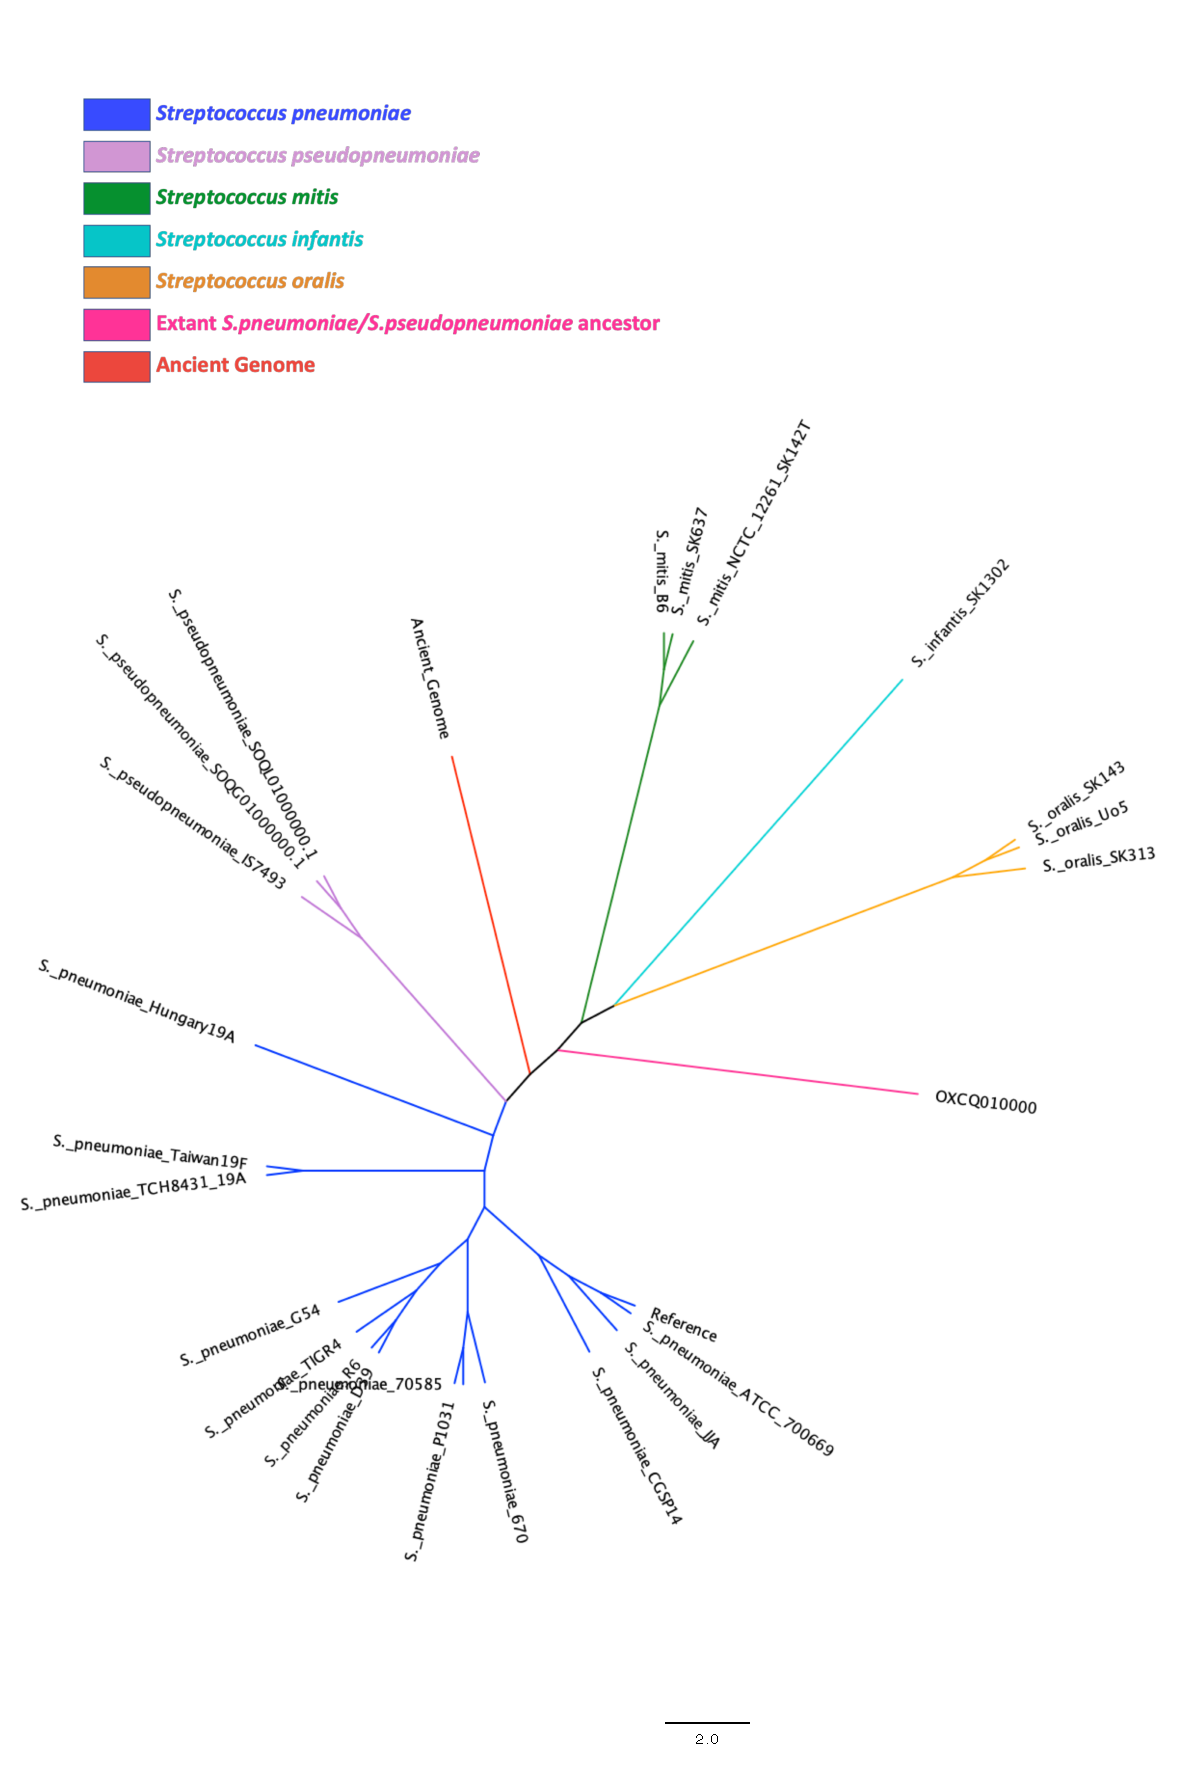
\includegraphics[width=\textwidth]{newMRCA.pdf}
    \caption{Contextualization of 5700 year old genome among extant pneumococcal and mitis group species including \textit{Streptococcus pneumoniae}(blue), \textit{Streptococcus pseudopneumoniae}(purple), \textit{Streptococcus mitis}(green),\textit{Streptococcus infantis} (turquoise), \textit{Streptococcus oralis}(orange), an extant \textit{Streptococcus pneumoniae}/\textit{Streptococcus pseudopneumoniae} ancestor (pink), and the ancient genome (red). This tree was built with iqtree with 1000 bootstraps and a GTR model. Visualized as an unrooted tree.}
      \label{fig:extantancient}
\end{figure}
1180/1000 words
\section{Discussion}
We have quantified estimates of geographic spatial structure of pneumococcal populations overall in South Africa. This provides a baseline for understanding geographic spread of individual phenotypes, as well as variability between countries Utilizing this odds ratio framework we were able to describe the effect of time and different geographic scales on pneumococcal spread.  We were able to mitigate the effect of spatial or sampling biases by restricting pairs to the same collection year; and this method has the potential to further mitigate other biases such as clinical manifestation or sampling site. We have shown that the strain designations (GPSCs) are sufficient to elucidate spatial structure and that it is 1.30 (95\% CI 1.18- 1.43) times more likely that a pair of isolates within a province will be the same GPSC as a pair from different provinces. This further validates the use of the PopPunk classification method which utilizes genetic distances across the entire genome for clustering \cite{leesFastFlexibleBacterial2019}. It also confirms the suspicion that there are distinct population ecology in different regions, even within the same country. The scale of this spatial effect varies by province and as yet we have not correlated this with any meaningful demographic or economic cause. Further evaluation of connectivity of provinces may elucidate a clearer mechanistic explanation. 
 \\The 54.28 (95\% CI 45.69-67.11) km/year rate of geographic spread estimated by our analysis implies that from the beginning of a year to the end of a year a strain will have transmitted approximately 54km. This is a rough estimate based on an isotropic transmission model. The key assumptions of this model which the pneumococcus violates include an equal mean and standard deviation, and infinite geographic distance. Neither of these assumptions are true as 1) it is likely that some transmission chains will extend further geographically, over a short period of time than others depending upon the mobility of the individual, and the propensity for transmission of the specific strain and 2) we are using a data set which is limited by the diameter of South Africa so the possible geographic distances between pairs are truncated. The rate of geographic spread could be used to predict the impact of the genetic backbone of a phenotype on its likely expansion time as well as the impact of location of emergence. However, our ability to determine if there is variable rate of geographic spread between GPSCs using this model is limited by the violation of assumptions. 
 \\Our determination of time to homogenization of strains across South Africa provides the first description of the rate of geographic, pneumococcal spread. Similar analysis has been done previously for dengue virus in Thailand \cite{saljeDengueDiversitySpatial2017} and the bacteria \textit{Listeria monocytogenes} in France \cite{mouraEmergenceGlobalSpread2020}. \textit{S. pneumoniae} moves at a slower geographic rate than either of these. 
\\The projected increasing growth of sub-Saharan African populations further highlights the need to understand the rate and mechanistic drivers of pneumococcal spread across geographic space \cite{abubakarFutureMigrationHuman2020a}. Overcrowding has been previously identified as a risk factor for pneumococcal pneumonia and a growing human host population will likely have implications for transmission and selection so understanding the baseline rates of geographic spread will be crucial for adapting treatment and prevention strategies \cite{veraniRiskFactorsPresumed2016}. 
 \\A limitation to this phylogeographic analysis is the true accuracy of time resolved phylogenies for \textit{S. pneumoniae}. Comparisons of patrisitic distances between BactDating and BEAST using relaxed and strict clock models, and a Bayesian skyline prior have $R^2$ values ranging from ~0.3 - ~0.9.  We are currently running BEAST and BactDating in multiple iterations to compare the clock rate models and priors. This will help to inform which software and models have the least uncertainty and highest accuracy time estimates between pairs. I am currently intending to move forward by imposing the BEAST estimated clock rate on BactDating as BEAST samples from a distribution of trees and is superior at determining a more accurate clock rate, while BactDating is better suited to the computational requirements of large bacterial data sets. Having greater confidence in the timed distances between pairs will help to confirm the results reported here and ensure that both our methods and results are robust as we move forward. 
\\The identification of a previously undescribed ancient streptococcal species does not benefit time resolution of GPSC phylogenies or elucidate further which GPSCs may have been circulating for longer periods than others. Its lack of capsule, however, does inform theories regarding evolution of mitis group capsular regions which have direct impacts on carriage duration and transmission propensity. The lack of a capsule in a \textit{S. pseudopneuoniae}/\textit{S. pneumoniae} ancestor implies acquisition and loss of the cps locus multiple times throughout streptococcal evolution. Non-encapsulated pneumococcal strains seem to have shorter carriage duration than their capsulated counterparts and this alongside carriage duration's inverse relationship with transmission may imply evolving streptococcal transmission rates over time\cite{bradshawSelectivePressureRise2019
bradshawTransformationNonencapsulatedStreptococcus2020}. Understanding the historic evolution may inform what could happen as the pneumoccocus continues to evolve, and new strains and phenotypes emerge.
819/900 words
\section{Future Work}
\subsection{Chapter 1: Describing the rate of pneumococcal geographic spread}
Thus far I have done a descriptive analysis of spatiotemporal dynamics of the pneumococcus in South Africa. I have answered the question "What is the rate of pneumococcal geographic spread and time to mixing in a population?" for South Africa specifically. \\Moving forward with this analysis I am looking to estimate the rate of geographic spread of individual GPSCs. I attempted to apply the same isotropic transmission model I applied overall (Figure \ref{fig:timedistance}A) to individual GPSCs (Figure \ref{fig:timedistance}B)  which, unfortunately, resulted in a sub-optimal model fit possibly as a result of the violation of assumptions as mentioned in the discussion. Quantifying the rate of geographic spread of different GPSCs can have major implications for understand how emerging phenotypes might spread through populations depending upon the backbone they have a propensity for. I plan to continue to modify my model to account for geographic truncation and unequal means and standard deviation.\\ Furthermore, whether the calculation of geographic rate of spread in South Africa is robust to different sampling resolutions remains unanswered. I will apply the same odds ratio framework to different geographic regions with both similar and higher resolution of geographic sampling coordinates. I have begun this by applying the same method to France with regards to a specific GPSC (10) and serotypes (24F) and it elucidated a shorter time to homogenization, as expected for a smaller geographic area. 
\subsection{Chapter 2: Obtaining a mechanistic understanding of transmission}
In the next phase of my analysis I will work towards obtaining a mechanistic understanding of what is driving geographic spread of the pneumococcus. To determine drivers of the rate of geographic spread I will include a probabilistic inference framework which includes time resolved phylogenies, number of transmissions inferred from the estimated generation time distribution and phylogenies, as well as a transition matrix. The transition matrix is key to understanding the most probable paths of transmission and utilizes matrix multiplication to incorporate all possible paths between all nine provinces of South Africa. Using this framework I can investigate likely paths of transmission through South Africa and then work towards identifying correlates to transmission which may include GPSC, serotype, population size, road or flight density, among other possible covariates\cite{saljeReconstructingUnseenTransmission2020a}.
\subsection{Chapter 3: Reconstructing previous long range transmission}
A different method which could elucidate similarly mechanistic drivers of pneumococcal transmission is a python implemented framework msprime which implements forward simulation in a stepping stone model of migration between clustered geographic locations (demes). Using this framework I will work to reconstruct previous long range transmission events and determine probable "highways" of transmission and their correlates such as: population size, density, or other demographic or economic factors. The nine provinces of South Africa will be discrete demes and similarly to the previously described method, there are multiple possible paths of transmission between each of these. Rather than using the entire pneumococcal pangenome I will select genes which are likely to have high prevalence in all populations, undergo negative selection and neutral evolution, slow enough to inform the migration model about the differences between two demes while not so slow that all genotypes between demes are identical. The current candidate subset for this are core metabolic genes which have been identified and annotated in a previous analysis of the GPS data set. To inform whether SNP allele frequencies are locally specific or spread across all populations I will plot SNP allele frequencies by GPSC and South African province. If these fall within goldilocks diversity between locations I will move forward with developing the model. Ultimately the goal is to reconstruct and determine the mechanistic drivers of likely migration routes and rates between geographic locations \cite{kelleherEfficientCoalescentSimulation2016,gutenkunstInferringJointDemographic2009}. 
\subsection{Chapter 4: History}
By analyzing an ancient pneumococcal genome I was hoping to determine which extant pneumococcal strains have emerged more recently and which may have been circulating for longer periods of time. The ancient genome analysis I undertook, however, resulted instead in identification of a novel species with a proposed name \textit{Candidatus} Streptococcus syltholmis. I have attached a draft of this paper in my supplement. \\The question of which strains have been circulating for longer and which have emerged more recently is still a question I am an interested in returning to. What it requires is accurate dating of phylogenies and incorporation of expansive diveristy into these dates. This is currently computationally intractable but I have hypothesize it may be possible once the variable rates of geographic transmission and clock rates between GPSCs have been determined. It is intractable using existing phylogenetic methods to determine time to divergence between pneumococcal sequence clusters. I hope to return to this question and interrogate methods, including graph based methods and SNP distance matrices to try to answer this.
\subsection{Chapter 5: Prediction}
If we successfully estimate variable rates of spread between GPSCs and the mechanistic drivers of predominant migratory paths we will have lay the groundwork for prediction. Ultimately, the ability to estimate the likely impact of introduction of a new or emerging phenotype to a geographic location will have great implications for treatment and prevention policy. 
820/1000 words
\section{Gantt Chart}
\begin{figure}
\centering
    \rotatebox{90}{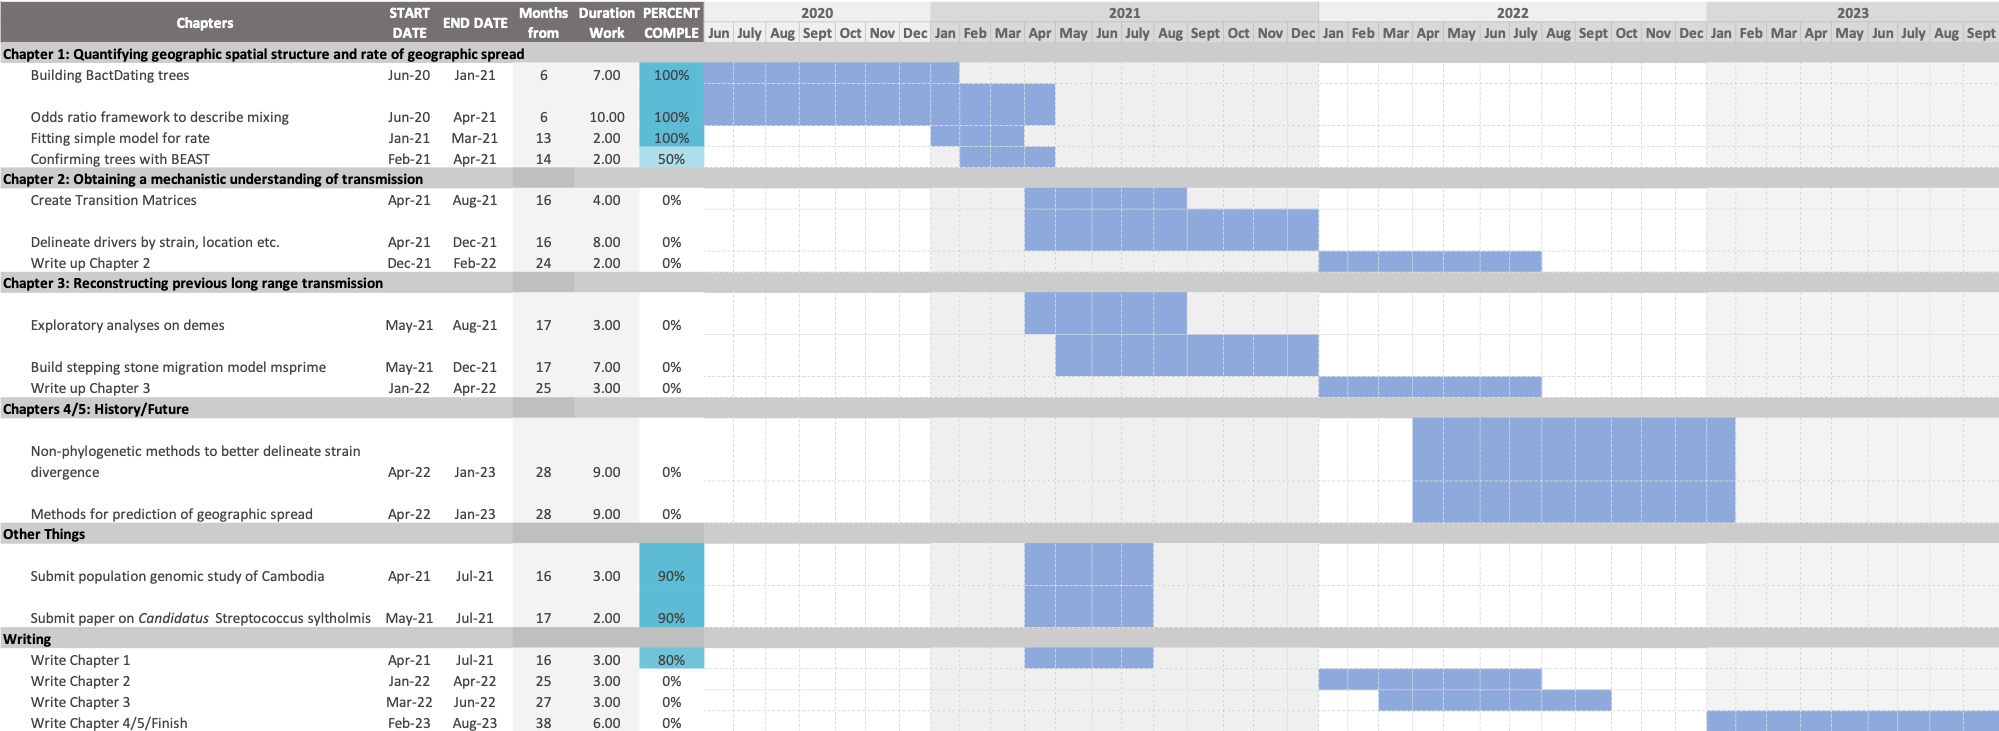
\includegraphics[width=\textheight]{ganttchart.png}}
    \caption{Draft of Gantt chart for remainder of PhD.}
      \label{fig:gantt}
\end{figure}
\printbibliography
\end{document}